%% ------------------------------------------------------------------------- %%
\chapter{Introdução}
\label{cap:introducao}

Test-Driven Development (TDD) é uma das práticas discutidas pela Programação
Extrema (XP) \cite{XPExplained}. A prática é baseada em um pequeno ciclo de
desenvolvimento, na qual o desenvolvedor deve sempre escrever um teste antes
mesmo de implementar a funcionalidade esperada, e depois, com o novo teste
passando, o desenvolvedor deve refatorar para remover duplicação
\cite{TDDByExample}.
Apesar da constante escrita de testes automatizados, os benefícios da prática 
vão além disso. Na opinião de muitos autores conhecidos, TDD promove
simplicidade, foco, melhor design, entre outras \cite{TDDByExample}
\cite{GOOS} \cite{astels-tdd}.

Por esses motivos, é possível observar a crescente adoção e procura por TDD
através do número de pesquisas publicadas pela academia.
Em um questionário de 2010, organizado por Scott Ambler
\cite{wambler-survey-agile}, para descobrir que práticas eram feitas por times
ágeis, mostrou que 53\% dos times ágeis adotaram TDD como uma maneira para
validar o trabalho feito, conforme mostra a Figura \ref{fig:wambler-agile-2010}. 
Outro questionário de 2008 também realizado por Ambler
\cite{wambler-survey-tdd}, focado em TDD, mostra que 57\% dos desenvolvedores 
utilizam TDD como técnica para capturar informações de design, conforme mostrado
na Figura \ref{fig:wambler-tdd-2008}.

No Brasil, é possível observar o crescente número de pessoas atrás de
informações sobre a prática nas mais diversas listas de discussão e fóruns sobre
tecnologia, como o GUJ \footnote{\url{http://www.guj.com.br}.
Último acesso em 27 de fevereiro 2011} ou o .NET Architects 
\footnote{\url{http://www.dotnetarchitects.net/}. Último acesso em
27 de fevereiro de 2011}. Diversos eventos de desenvolvimento de
software realizados no Brasil em 2010, como a QCON SP
\footnote{\url{http://www.qconsp.com/}. Último acesso em 02 de março de 2011} e
a Agile Brazil \footnote{\url{http://http://www.agilebrazil.com/}. Último acesso
em 02 de março de 2011} também contaram com palestras sobre o assunto.

Os aficionados por TDD dizem que estão \textit{``infectados pelo teste''}  e,
segundo eles próprios, desenvolvedores que experimentam a prática e percebem
seus efeitos tendem a não voltar atrás \cite{tdd-fearless}.
Já Robert Martin relaciona TDD à profissionalismo. Segundo ele, um desenvolvedor
profissional entrega código claro e flexível que funcione dentro do prazo, e TDD
possibilita que o desenvolvedor alcance esses pontos \cite{martin-profissionalismo}.

Discutir os efeitos de TDD no design de classes é de grande importância para os
desenvolvedores.
Criar classes ou, em um nível maior de abstração, módulos que possuam um baixo
acoplamento e uma alta coesão demandam um esforço muito grande do desenvolvedor. 
É muito comum que, após algum tempo de desenvolvimento, o design perca qualidade
e qualquer tipo de manutenção torne-se difícil e, por consequência, custosa.
Para diminuir o problema, desenvolvedores utilizam diversas práticas para
garantir a qualidade do código gerado, como programação pareada, revisão de
código, etc. Praticantes de TDD acreditam que os testes sejam uma outra maneira
de validar o design criado, e utilizar esse feedback para melhorá-lo.

É realmente difícil entender como TDD influencia no processo de desenvolvimento
de software, e mais especificamente no design de classes. Grande parte dos
experimentos feitos pela academia verificam os efeitos da prática sobre a qualidade externa. 
Poucos são os estudos que avaliam TDD do ponto de vista da qualidade interna de
código. Siniaalto e Abrahamsson também compartilham dessa opinião e, além disso,
notaram que os efeitos de TDD podem não ser tão automáticos ou evidentes como o 
esperado \cite{alarming-results}.

Relacionar o fato do desenvolvedor escrever testes antes e, por esse motivo,
levar o design para melhores soluções não é trivial.
Este trabalho visa compreender os efeitos e como a prática de TDD
influencia no design de sistemas orientados a objetos do ponto de vista dos
desenvolvedores que a praticam. Para alcancar esse objetivo,
esta pesquisa discute três estudos de caso em empresas do mercado brasileiro de
software, que já utilizam TDD normalmente dentro do seu ciclo de
desenvolvimento. Para isso, este trabalho faz uso de métodos qualitativos de
pesquisa, melhor explicados no Capítulo \ref{cap:planejamento}.

\begin{figure}[ht]
  \begin{minipage}[b]{0.45\linewidth}
    \centering
    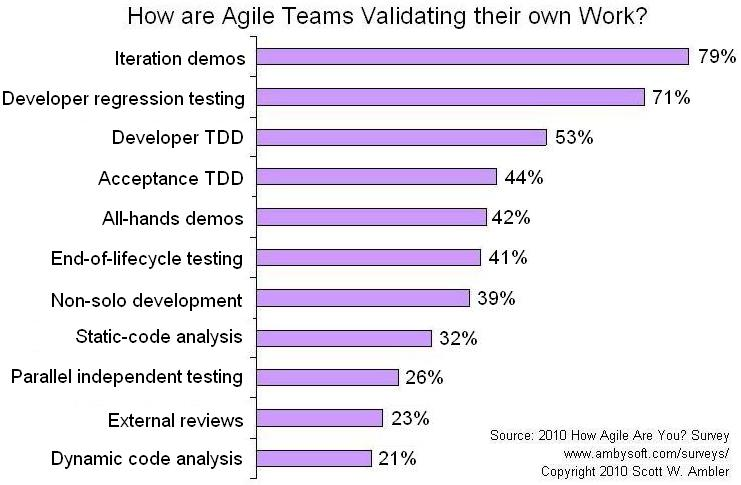
\includegraphics[scale=.4]{agileCriteria2010Validating}
    \caption{Como times ágeis validam seu próprio trabalho?}
    \label{fig:wambler-agile-2010}
  \end{minipage}
  \hspace{0.5cm}
  \begin{minipage}[b]{0.45\linewidth}
    \centering
    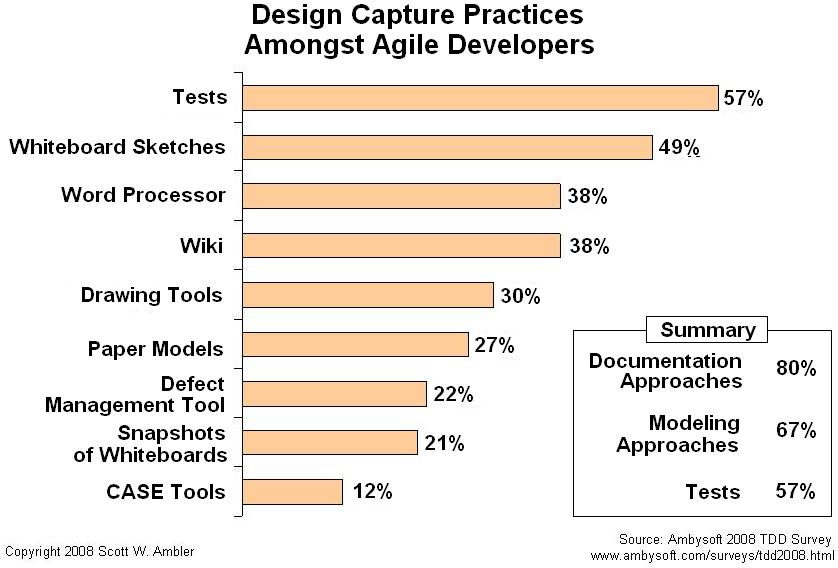
\includegraphics[scale=.35]{tddDesignPractices}
    \caption{Maneiras de captura de design entre desenvolvedores ágeis}  
    \label{fig:wambler-tdd-2008}
  \end{minipage}
\end{figure}			

%% ------------------------------------------------------------------------- %%
\section{Contribuições}

O objetivo desta pesquisa é entender como TDD influencia no design de sistemas
orientados a objetos. A análise será feita através de dados que serão
capturados baseados na percepção de programadores que realizam a prática no seu
dia-a-dia de trabalho.
Os objetivo principal da pesquisa é \textbf{entender a influência de TDD no
design de sistemas orientados a objetos}.

Como mencionado acima, praticantes de TDD afirmam que a prática os ajuda a criar
classes que apresentam simplicidade, baixo acoplamento e alta coesão. Para
compreender esses efeitos, essa pesquisa tenta responder as questões listadas
abaixo:

\begin{itemize}

  \item Como a prática de TDD afeta o acoplamento das classes criadas?

  \item Como a prática de TDD afeta o gerenciamento de dependências em sistemas
  orientados a objetos?

  \item Como a prática de TDD afeta a coesão das classes criadas?

  \item Como TDD afeta a simplicidade das classes criadas?

  \item Como o teste guia o desenvolvedor durante a atividade de
  design?

\end{itemize}

%% ------------------------------------------------------------------------- %%
\section{Organização do trabalho}

Este trabalho está dividido da seguinte maneira: 

\begin{itemize}
	\item O Capítulo \ref{cap:tdd} discute sobre a prática de TDD, com ênfase no
	ponto de vista do design.
  
	\item O Capítulo \ref{cap:trabalhos-relacionados} mostra trabalhos já
	realizados pela academia sobre os efeitos de TDD.
	
	\item O Capítulo \ref{cap:discussao} apresenta os resultados encontrados e
	discute em cima dos mesmos.
	
	\item O Capítulo \ref{cap:ameacas} discute as possíveis ameaças dos resultados
	encontrados na pesquisa.
	
	\item O Capítulo \ref{cap:conclusoes} resume o trabalho realizado a apresenta
	possibilidades de trabalhos futuros.
\end{itemize}
